\documentclass{article}
\usepackage{graphicx}
\usepackage{amsmath}
\usepackage{amsfonts}
\usepackage{bookmark}
\usepackage{booktabs}
\usepackage{exercises}
\graphicspath{ {./images/4.7} }
\usepackage{indentfirst}
\usepackage{amsthm}
\usepackage{yhmath}
\usepackage{placeins}
\newcommand*{\oldneg}{\mathord{\sim}}
\newcommand\showdiv[1]{\overline{\smash{)}#1}}
\newcommand\Mydiv[1]{%
\smash{\raise.3ex\hbox{$\big)$}}\mkern-8mu
        \overline{\enspace\strut#1}}
\setlength{\tabcolsep}{5pt}
\theoremstyle{definition}
\newtheorem{definition}{Definition}

\setlength{\parindent}{.5in}
\setlength{\parskip}{12pt}
\renewcommand{\arraystretch}{2}
\newcommand{\?}{\stackrel{?}{=}}

\title{4.7 Answers}
\begin{document}
\maketitle

\section*{1}
Given a set of more than two data pairs $(x,y)$, you can decide whether an exponential function fits the data well by 
making a scatter plot of the points $(x,\ln y)$.

\section*{2}
Suppose that we are given set of data pairs $(x,y)$. To tell if the power function fits the data well, 
we first graph the points $(\ln x,\ln y)$. Then, we determine how close those points come to being linear. If they are linear, we know that 
the data fits a power function. If it is not linear, we know that it does not fit a power function.

\section*{10}
We know that \[ 6.4=ab^2,409.6=ab^5 \] thus meaning \[ a=\frac{6.4}{b^2} \]
We can then solve for $a$ and $b$:
\[ 409.6=\frac{6.4}{b^2}b^5=6.4b^3 \] \[ 64=b^3 \] \[ b=4 \] meaning \[ a=\frac{6.4}{4^2}=\frac{6.4}{16}=0.4 \]
Thus, the exponential function matching this data is:
\[ y=0.4\times 4^x \]

\section*{14}
We are given the set of data:
\[ (1,1.4),(2,6.7),(3,32.9),(4,161.4),(5,790.9) \] We must graph the points:
\[ (1,0.34),(2,1.90),(3,3.49),(4,5.08),(5,6.67) \] Now, if these points were linear, the slope would be about:
\[ \dfrac{0.34-1.90}{1-2}=1.56 \] meaning an equation for that line would be about:
\[ \ln y-1.90=1.56(x-0.34) \] where $y$ is the $y$-value of the first data set:\newline
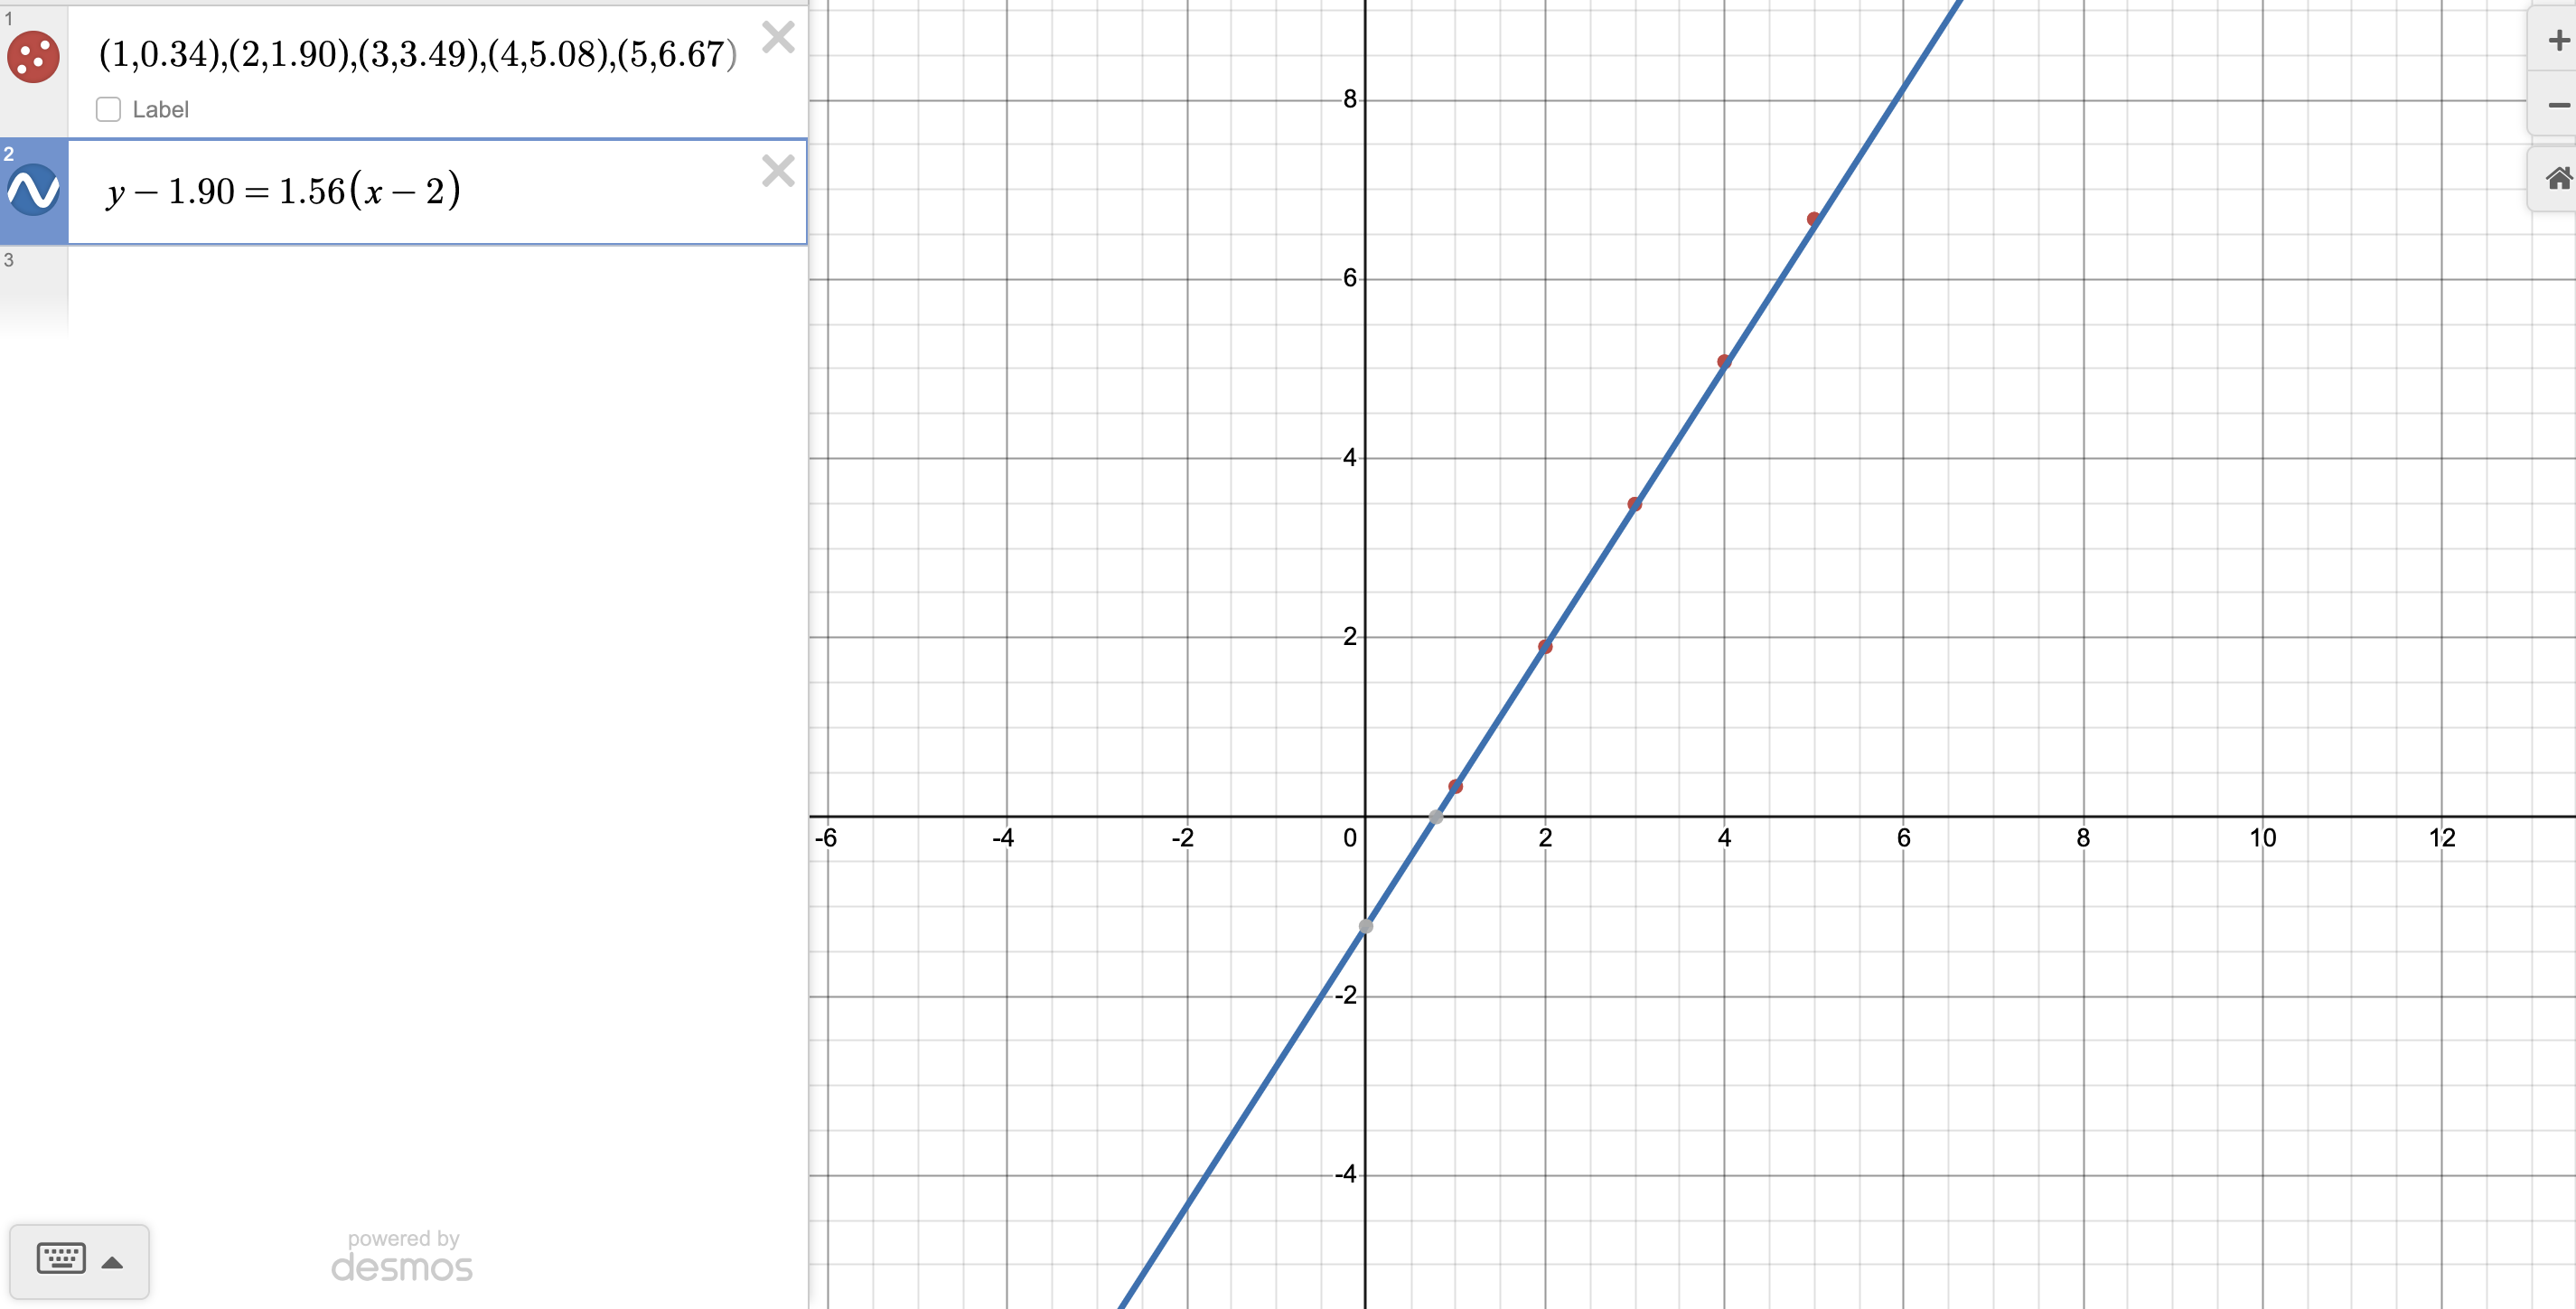
\includegraphics[width = 4in, height = 4in]{14}\newline
which appears to be linear. Thus, we can solve the equation (remembering that $\ln y$ is our output with regards to the first data set):
\[ \ln y-1.90=1.56(x-0.34) \] \[ \ln y=1.56x+1.3696 \] \[ y=e^{1.56x+1.3696} \] \[ y=e^{1.3696}(e^{1.56})^x \]
\[ y=3.93(4.76)^x \]

\section*{22}
We know that \[ 5=a(3.1)^b,9.7=a(6.8)^b \] meaning \[ a=\dfrac{5}{3.1^b} \]
We can then solve for $a$ and $b$:
\[ 9.7=\dfrac{5}{3.1^b}(6.8)^b \] \[ 9.7\approx 5\times 2.19^b \] \[ 1.94=2.19^b \] \[ \log_2.19 1.94=\log_2.19 2.19^b \]
\[ \dfrac{\log 2.19}{\log 1.94}=b \] \[ b\approx 1.18 \] 
meaning \[ a\approx \dfrac{5}{3.1^{1.18}}\approx 1.32 \]
meaning the power function matching this data is:
\[ y=1.32x^{1.18} \]

\section*{26}
We are given the set of data:
\[ (1,0.81),(2,0.99),(3,1.11),(4,1.21),(5,1.29) \]
We must graph the points:
\[ (0,-0.21),(0.69,-0.01),(1.10,0.10),(1.39,0.19),(1.61,0.25) \]
If these points were linear, the slope would be about:
\[ \dfrac{0.10+0.21}{1.10-0}\approx 0.28 \] meaning an equation for that line would be about:
\[ \ln y+0.21=0.28\ln x \]
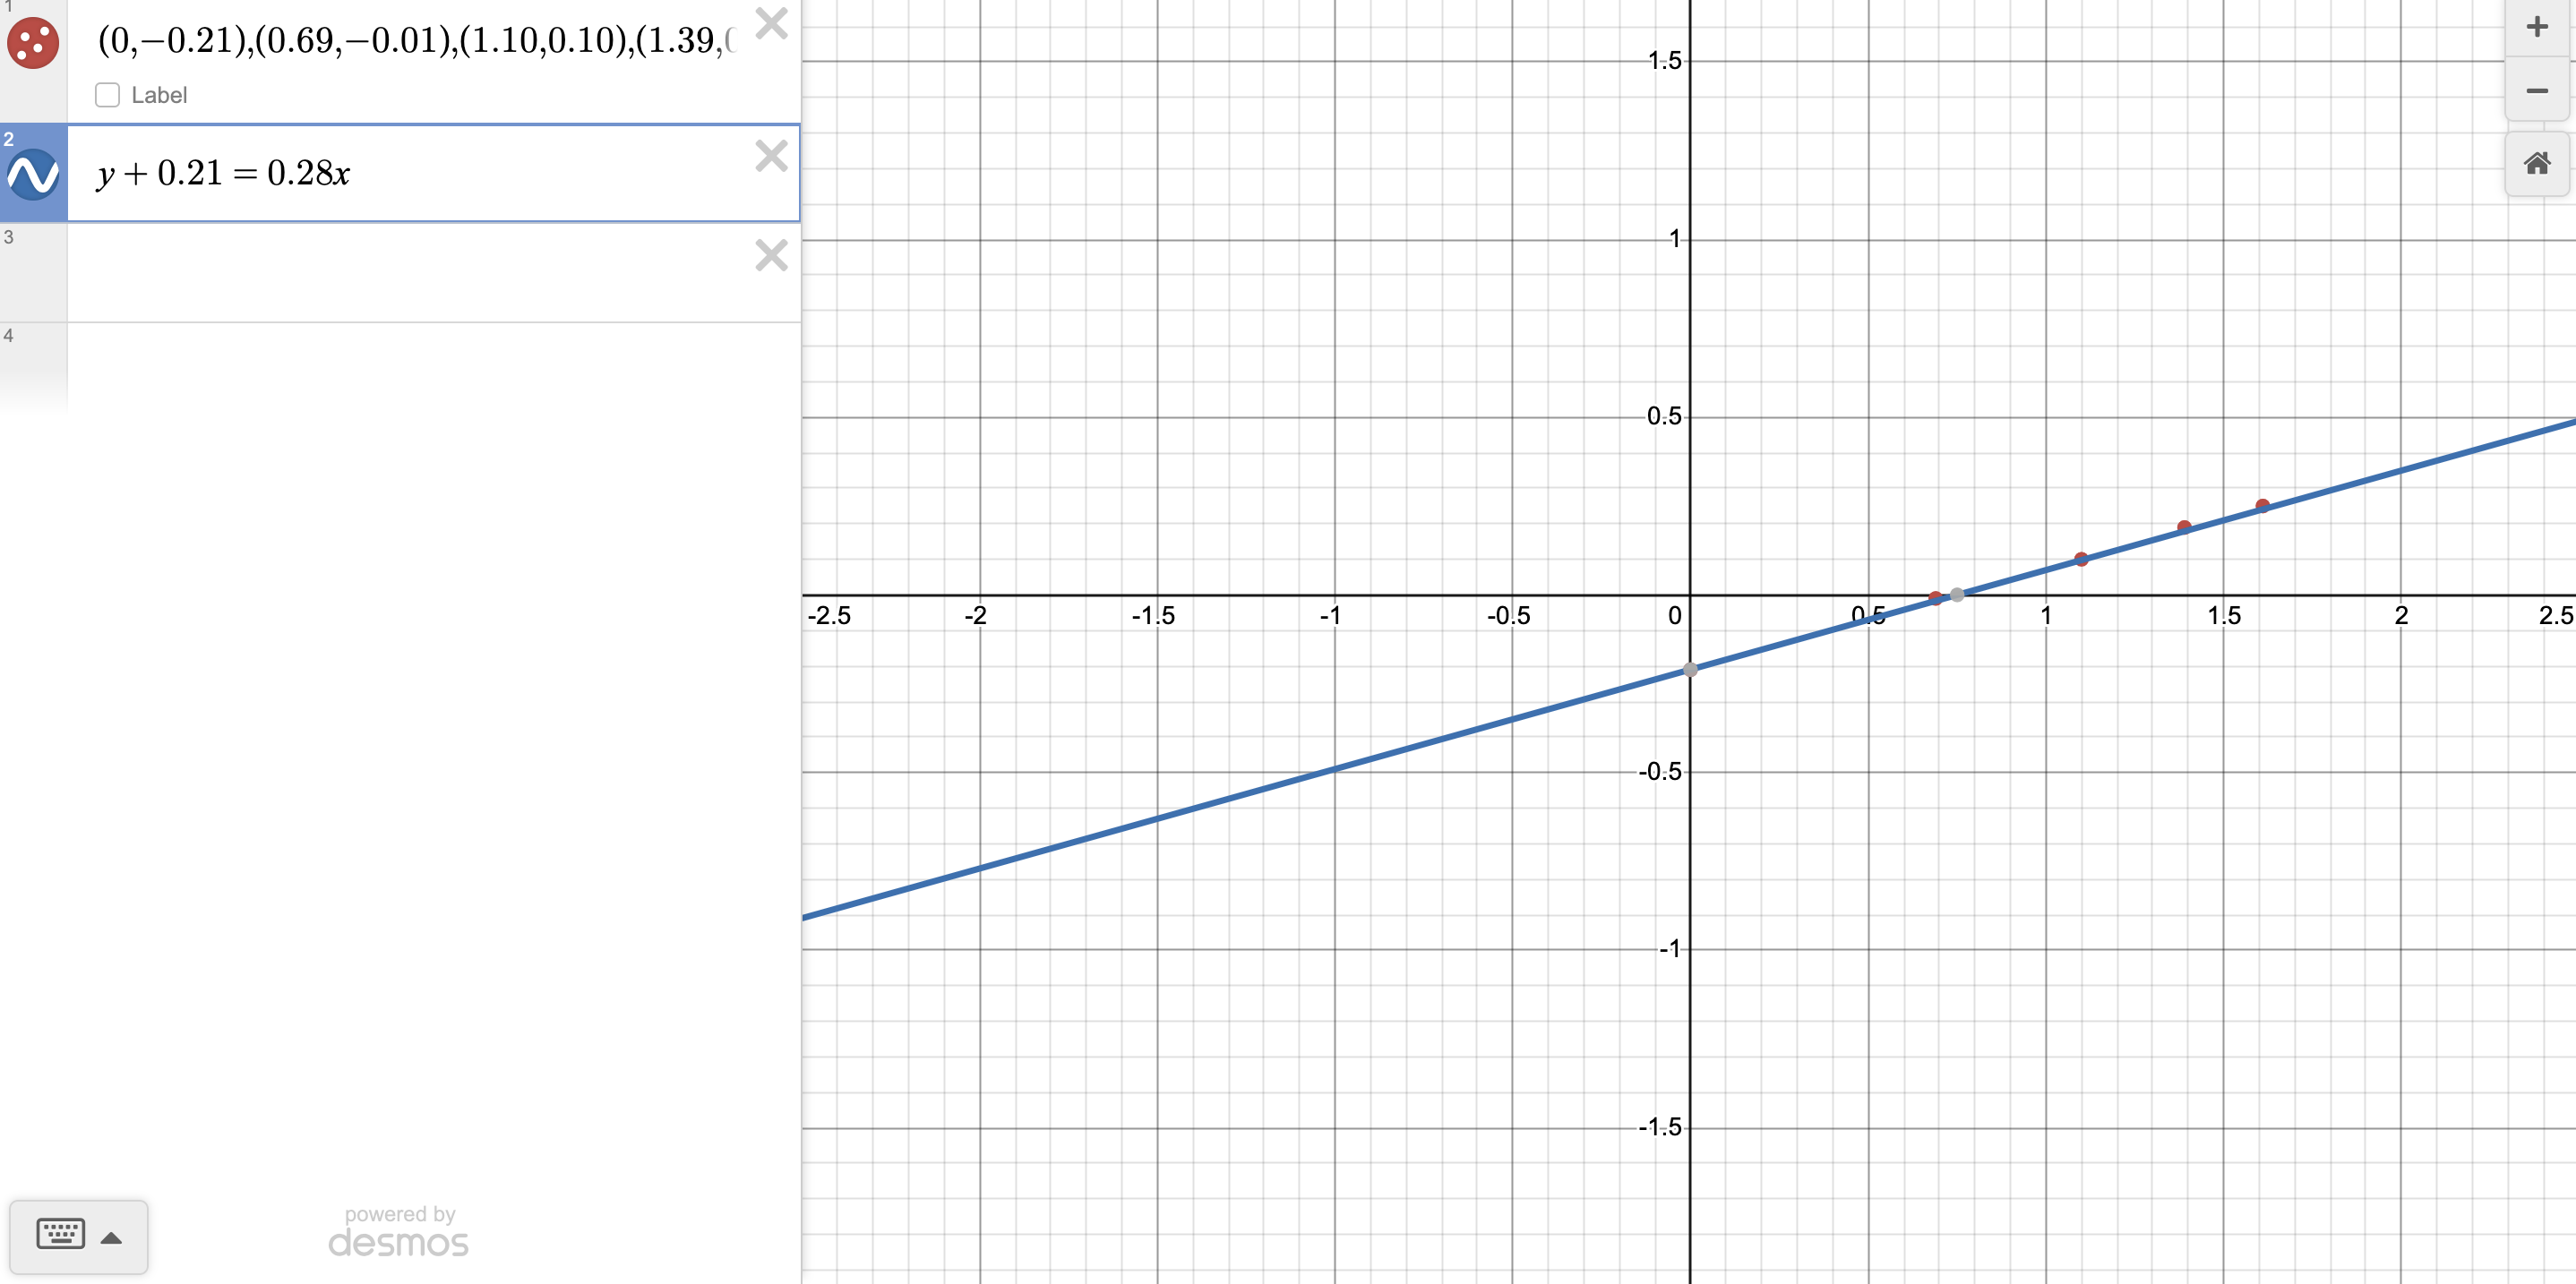
\includegraphics[width = 4in, height = 4in]{26}\newline
which appears to be linear. Thus, we can solve the equation:
\[ \ln y+0.21=0.28\ln x \] \[ \ln y=0.28\ln x-0.21 \] \[ e^{\ln y}=e^{0.28\ln x-0.21} \] \[ y=e^{-0.21}(e^{\ln x})^{0.28} \]
\[ y=0.81(x)^{0.28} \]

\section*{27}
A

\section*{28}
The error here is on the third line $e^{2x+1}$ is not equal to $e^{2x}+e^1$, but rather $e^{2x}\times e^1$. Thus:
\[ \ln y=2x+1 \] \[ y=e^{2x+1} \] \[ y=e^{2x}\times e^1 \] \[ y=e(e^2)^x \] \[ y=2.72(7.39)^x \]

\section*{30}
(a): \[ y=ab^x \] \[ \ln y=\ln\left(ab^x\right) \] \[ \ln y=\ln a+\ln\left(b^x\right) \] \[ \ln y=\ln a+x\ln b \]
This means that slope of the line relating $x$ and $\ln y$ in the above equation is $\ln b$, while the $y$-intercept is $\ln a$.


(b): \[ y=ax^b \] \[ \ln y=\ln\left(ax^b\right) \] \[ \ln y=\ln a+\ln\left(x^b\right) \] \[ \ln y=\ln a+b\ln x \]
meaning the slope of the line relating $\ln x$ and $\ln y$ in the above equation is $b$, while the $y$-intercept is $\ln a$.

\end{document}

